\chapter{System analysis}
\label{ch:system_analysis}

\section{Analysis of the dataset}
\label{sec:dataset_analysis}

\subsection{About the dataset}
\label{subsec:about_dataset}

The empirical foundation of the ClauseIQ platform is derived from the Contract Understanding Atticus Dataset (CUAD v1), created by The Atticus Project and curated by legal scholars and practicing commercial attorneys~\cite{hendrycks2021cuad}. CUAD was assembled to provide an open, standardized, and rigorous benchmark for legal document comprehension, contract review automation, and clause information extraction. The underlying corpus comprises \TotalContracts{} comprehensive commercial contracts filed with the United States Securities and Exchange Commission (SEC) via its Electronic Data Gathering, Analysis, and Retrieval (EDGAR) database.

In its raw distribution, CUAD provides document-level JSON annotations organized according to the Stanford Question Answering Dataset (SQuAD 2.0) format. Each annotation specifies start and end character offsets of contractual provisions mapped across \NumClasses{} legal categories. For supervised classification and intelligent semantic retrieval, the raw annotations were systematically parsed, validated, and consolidated into a tabular schema. The finalized clean corpus, stored at \path{data/clauseiq_dataset_clean.csv}, consists of \TotalClauses{} verified clause rows across three core columns: \texttt{contract\_id}, \texttt{clause\_text}, and \texttt{category}.

A data integrity audit conducted by \path{report/scripts/make_numbers.py} confirms:
\begin{itemize}
    \item Completeness: Across all \TotalClauses{} records, there are exactly \NullValueCount{} null, missing, or undefined values. Every record contains a valid contract identifier, populated clause text, and standardized category string.
    \item Distinct parent contracts: The clauses originate from \TotalContracts{} distinct commercial agreements, ensuring broad organizational, jurisdictional, and industrial representation across mergers and acquisitions, joint ventures, software licensing, commercial leases, and supply agreements.
    \item Categorical coverage: Exactly \NumClasses{} standardized legal categories are populated, ranging from foundational transactional provisions (such as \textit{Parties}, \textit{Agreement Date}, and \textit{Governing Law}) to specialized regulatory covenants (such as \textit{Anti-Corruption/FCPA}, \textit{Export Control}, and \textit{Volume Restriction}).
    \item Textual duplication and boilerplate: Exactly \DuplicateClauseCount{} clause texts appear more than once across distinct contracts. These identical entries represent universal legal boilerplate covenants (e.g., standard severability recitals, identical Delaware governing law clauses, and boilerplate counterpart execution provisions). Rather than discarding valid boilerplate instances, duplicate instances across distinct contracts are preserved to reflect real-world transactional drafting distributions.
\end{itemize}

\subsection{Explore the dataset}
\label{subsec:explore_dataset}

Quantitative inspection of the clause texts reveals significant variance in length, token density, and class representation. Table~\ref{tab:dataset_summary_statistics} summarizes the descriptive statistics computed across the \TotalClauses{} clauses.

\begin{table}[htbp]
\centering
\small
\begin{tabular}{lccccc}
\toprule
\textbf{Metric Attribute} & \textbf{Minimum} & \textbf{Maximum} & \textbf{Mean} & \textbf{Median} & \textbf{Std. Dev.} \\
\midrule
Clause Word Count (Tokens) & \MinWordCount{} & \MaxWordCount{} & \MeanWordCount{} & \MedianWordCount{} & \StdWordCount{} \\
Clause Character Length & \MinCharCount{} & \MaxCharCount{} & \MeanCharCount{} & \MedianCharCount{} & \StdCharCount{} \\
Clauses per Contract & \MinClausesPerContract{} & \MaxClausesPerContract{} & \MeanClausesPerContract{} & \MedianClausesPerContract{} & \StdClausesPerContract{} \\
\bottomrule
\end{tabular}
\caption{Descriptive statistical summary of the validated CUAD clause dataset}\label{tab:dataset_summary_statistics}
\end{table}

The shortest clauses in the corpus comprise just \MinWordCount{} tokens (such as brief date designations or party headings), while the longest provision spans \MaxWordCount{} words (\MaxCharCount{} characters), representing extensive, multi-sentence intellectual property licensing conditions. On average, commercial agreements yield \MeanClausesPerContract{} annotated clauses, though density ranges from \MinClausesPerContract{} clause in single-purpose amendment letters up to \MaxClausesPerContract{} clauses in highly negotiated joint venture charters.

The dataset exhibits substantial class imbalance. The most frequent category, \textit{\MostFrequentCategory{}}, contains \MostFrequentCategoryCount{} instances (10.25\% of the corpus), whereas the least frequent category, \textit{\LeastFrequentCategory{}}, contains only \LeastFrequentCategoryCount{} instances (0.22\% of the corpus). This yields an overall class imbalance ratio of \ImbalanceRatio{}. Table~\ref{tab:category_distribution} provides the complete distribution across all \NumClasses{} categories.

% Auto-generated by scripts/make_numbers.py
\begin{longtable}{r p{6.5cm} r r}
\toprule
\textbf{Rank} & \textbf{Category Name} & \textbf{Sample Count} & \textbf{Percentage (\%)} \\
\midrule
\endfirsthead
\multicolumn{4}{c}{{\bfseries Table \thetable\ continued from previous page}} \\
\toprule
\textbf{Rank} & \textbf{Category Name} & \textbf{Sample Count} & \textbf{Percentage (\%)} \\
\midrule
\endhead
\midrule
\multicolumn{4}{r}{{Continued on next page}} \\
\bottomrule
\endfoot
\bottomrule
\caption{Complete 41-category legal clause distribution in the cleaned CUAD corpus}\label{tab:category_distribution}\\
\endlastfoot
1 & Parties & 1,251 & 10.25\% \\
2 & License Grant & 774 & 6.34\% \\
3 & Cap On Liability & 672 & 5.51\% \\
4 & Anti-Assignment & 652 & 5.34\% \\
5 & Audit Rights & 642 & 5.26\% \\
6 & Insurance & 559 & 4.58\% \\
7 & Expiration Date & 467 & 3.83\% \\
8 & Governing Law & 462 & 3.79\% \\
9 & Post-Termination Services & 449 & 3.68\% \\
10 & Agreement Date & 426 & 3.49\% \\
11 & Minimum Commitment & 424 & 3.47\% \\
12 & Effective Date & 421 & 3.45\% \\
13 & Revenue/Profit Sharing & 417 & 3.42\% \\
14 & Exclusivity & 409 & 3.35\% \\
15 & Rofr/Rofo/Rofn & 367 & 3.01\% \\
16 & Ip Ownership Assignment & 317 & 2.60\% \\
17 & Document Name & 306 & 2.51\% \\
18 & Non-Transferable License & 295 & 2.42\% \\
19 & Non-Compete & 257 & 2.11\% \\
20 & Change Of Control & 253 & 2.07\% \\
21 & Termination For Convenience & 246 & 2.02\% \\
22 & Renewal Term & 209 & 1.71\% \\
23 & Warranty Duration & 175 & 1.43\% \\
24 & Covenant Not To Sue & 173 & 1.42\% \\
25 & Volume Restriction & 170 & 1.39\% \\
26 & Uncapped Liability & 167 & 1.37\% \\
27 & Irrevocable Or Perpetual License & 165 & 1.35\% \\
28 & Competitive Restriction Exception & 124 & 1.02\% \\
29 & Notice Period To Terminate Renewal & 121 & 0.99\% \\
30 & Liquidated Damages & 121 & 0.99\% \\
31 & Affiliate License-Licensee & 115 & 0.94\% \\
32 & Joint Ip Ownership & 115 & 0.94\% \\
33 & No-Solicit Of Employees & 91 & 0.75\% \\
34 & Affiliate License-Licensor & 69 & 0.57\% \\
35 & Source Code Escrow & 65 & 0.53\% \\
36 & Non-Disparagement & 64 & 0.52\% \\
37 & No-Solicit Of Customers & 58 & 0.48\% \\
38 & Third Party Beneficiary & 39 & 0.32\% \\
39 & Most Favored Nation & 38 & 0.31\% \\
40 & Unlimited/All-You-Can-Eat-License & 32 & 0.26\% \\
41 & Price Restrictions & 27 & 0.22\% \\
\midrule
& Total & 12,204 & 100.00\% \\
\end{longtable}


\section{Data preprocessing}
\label{sec:data_preprocessing}

\subsection{Data cleaning}
\label{subsec:data_cleaning}

Raw legal texts extracted from SEC EDGAR filings contain formatting noise, typographic artifacts, multi-byte Unicode inconsistencies, and structural irregularities. To ensure uniform input into feature extraction algorithms, a deterministic preprocessing pipeline was implemented in \path{src/text_cleaner.py} and executed via \path{src/build_artifacts.py}.

The cleaning pipeline executes the following sequential transformations:
\begin{enumerate}
    \item Unicode normalization: Converts non-standard whitespace characters (non-breaking spaces, zero-width spaces) and typographic quotes (e.g., smart quotes \texttt{``\,''} and dashes \texttt{---}) into standardized ASCII equivalents.
    \item Case normalization: Converts all textual input to lower-case characters, eliminating capitalization discrepancies across draft titles and paragraph headings.
    \item Noise and URL removal: Identifies and removes web URLs, email strings, and file-system artifacts using targeted regular expressions.
    \item Legal symbol preservation: Unlike general-purpose NLP tokenizers that strip all punctuation, the cleaning routine explicitly preserves semantically significant legal punctuation and numbering indicators (including section symbols \texttt{\S}, percentage signs \texttt{\%}, currency symbols, hyphens, and slashes) which delineate statutory references and sub-clause designations.
    \item Whitespace consolidation: Collapses irregular line feeds, carriage returns, tab characters, and multiple spaces into single space separators, trimming leading and trailing whitespace.
\end{enumerate}

\subsection{Analysis of feature variables}
\label{subsec:feature_analysis}

In natural language processing, textual sequences must be mapped into vector representations that capture syntactic structure and semantic intent. To identify the optimal feature extraction methodology for legal provisions, systematic cross-validation experiments were conducted on the training data, as logged in \path{results/experiments.csv}.

The empirical progression yielded critical architectural findings:
\begin{itemize}
    \item Impact of stopword removal (EXP-01C): Standard NLP preprocessing routinely discards English stopwords (such as ``shall'', ``may'', ``not'', ``unless'', ``if''). When evaluated on the CUAD corpus, removing standard NLTK stopwords caused 5-fold cross-validation Macro-F1 to decline from 0.6614 to 0.6567 (accuracy dropped from 74.30\% to 73.88\%). In legal drafting, modal auxiliary verbs convey fundamental jurisdictional meaning: ``shall'' denotes mandatory obligation, ``may'' indicates discretionary permission, and ``unless'' establishes conditional exemptions. Discarding these tokens degrades discriminative precision. Consequently, stopword removal was excluded from the final pipeline.
    \item Impact of lemmatization (EXP-01D): Applying NLTK WordNet lemmatization~\cite{bird2009natural} (\texttt{clean\_text\_lemmatized}) improved 5-fold cross-validation Macro-F1 from 0.6614 to 0.6662 and accuracy to 74.67\%. Lemmatization successfully collapses inflected legal variants (e.g., ``terminates'', ``terminating'', ``terminated'' $\rightarrow$ ``terminate'') without discarding semantic distinctions.
    \item Hybrid word and character n-gram feature union (EXP-02D): Expanding pure word vocabulary up to 50,000 features yielded diminishing returns (0.6636 Macro-F1 in EXP-02B). However, constructing a \texttt{FeatureUnion} combining 25,000 word n-grams (unigrams and bigrams) with 15,000 character n-grams within word boundaries (\texttt{char\_wb}, 3--5 character window) produced a major performance leap, elevating 5-fold cross-validation Macro-F1 to 0.6865 and accuracy to 76.18\%.
\end{itemize}

The finalized feature extraction architecture utilizes sublinear term frequency scaling ($1 + \log(TF)$) and inverse document frequency (IDF) weighting~\cite{salton1988term, manning2008introduction}, creating a 40,000-dimensional sparse feature space:
\begin{equation}
    TF\text{-}IDF(t, d, D) = \big(1 + \log(TF(t, d))\big) \times \log\left(\frac{1 + |D|}{1 + DF(t, D)}\right) + 1
    \label{eq:sublinear_tfidf}
\end{equation}
The inclusion of \texttt{char\_wb} n-grams provides robustness against spelling variants, compound legal affixes (e.g., ``indemn-'', ``licens-'', ``-ability''), and hyphenated legal terms.

\subsection{Analysis of class variables}
\label{subsec:class_analysis}

The target variable encompasses \NumClasses{} nominal legal categories. Prior to model training, the category strings are mapped into integer class labels $y \in \{0, 1, \dots, 40\}$ using scikit-learn's \texttt{LabelEncoder}~\cite{pedregosa2011scikit}.

To counteract the \ImbalanceRatio{} class imbalance ratio, all evaluated linear classifiers employ cost-sensitive balanced class weighting. The weight $w_c$ for class $c$ is calculated inversely proportional to its training frequency:
\begin{equation}
    w_c = \frac{N}{K \times N_c}
    \label{eq:class_weight}
\end{equation}
where $N$ is the total number of training clauses, $K = 41$ is the number of distinct categories, and $N_c$ is the number of training samples belonging to category $c$. Under this formulation, rare classes receive higher loss penalties during gradient updates, preventing optimization routines from ignoring low-frequency covenants.

\section{Data visualization}
\label{sec:data_visualization}

To illustrate corpus characteristics and validate engineering assumptions, visualizations were generated using \path{report/scripts/make_figures.py}.

Figure~\ref{fig:dataset_category_distribution} displays the frequency distribution across all \NumClasses{} legal categories. The distribution exhibits an exponential decay, with the top five categories accounting for over 30\% of total records, while the bottom ten categories each contain fewer than 100 samples.

\begin{figure}[htbp]
\centering
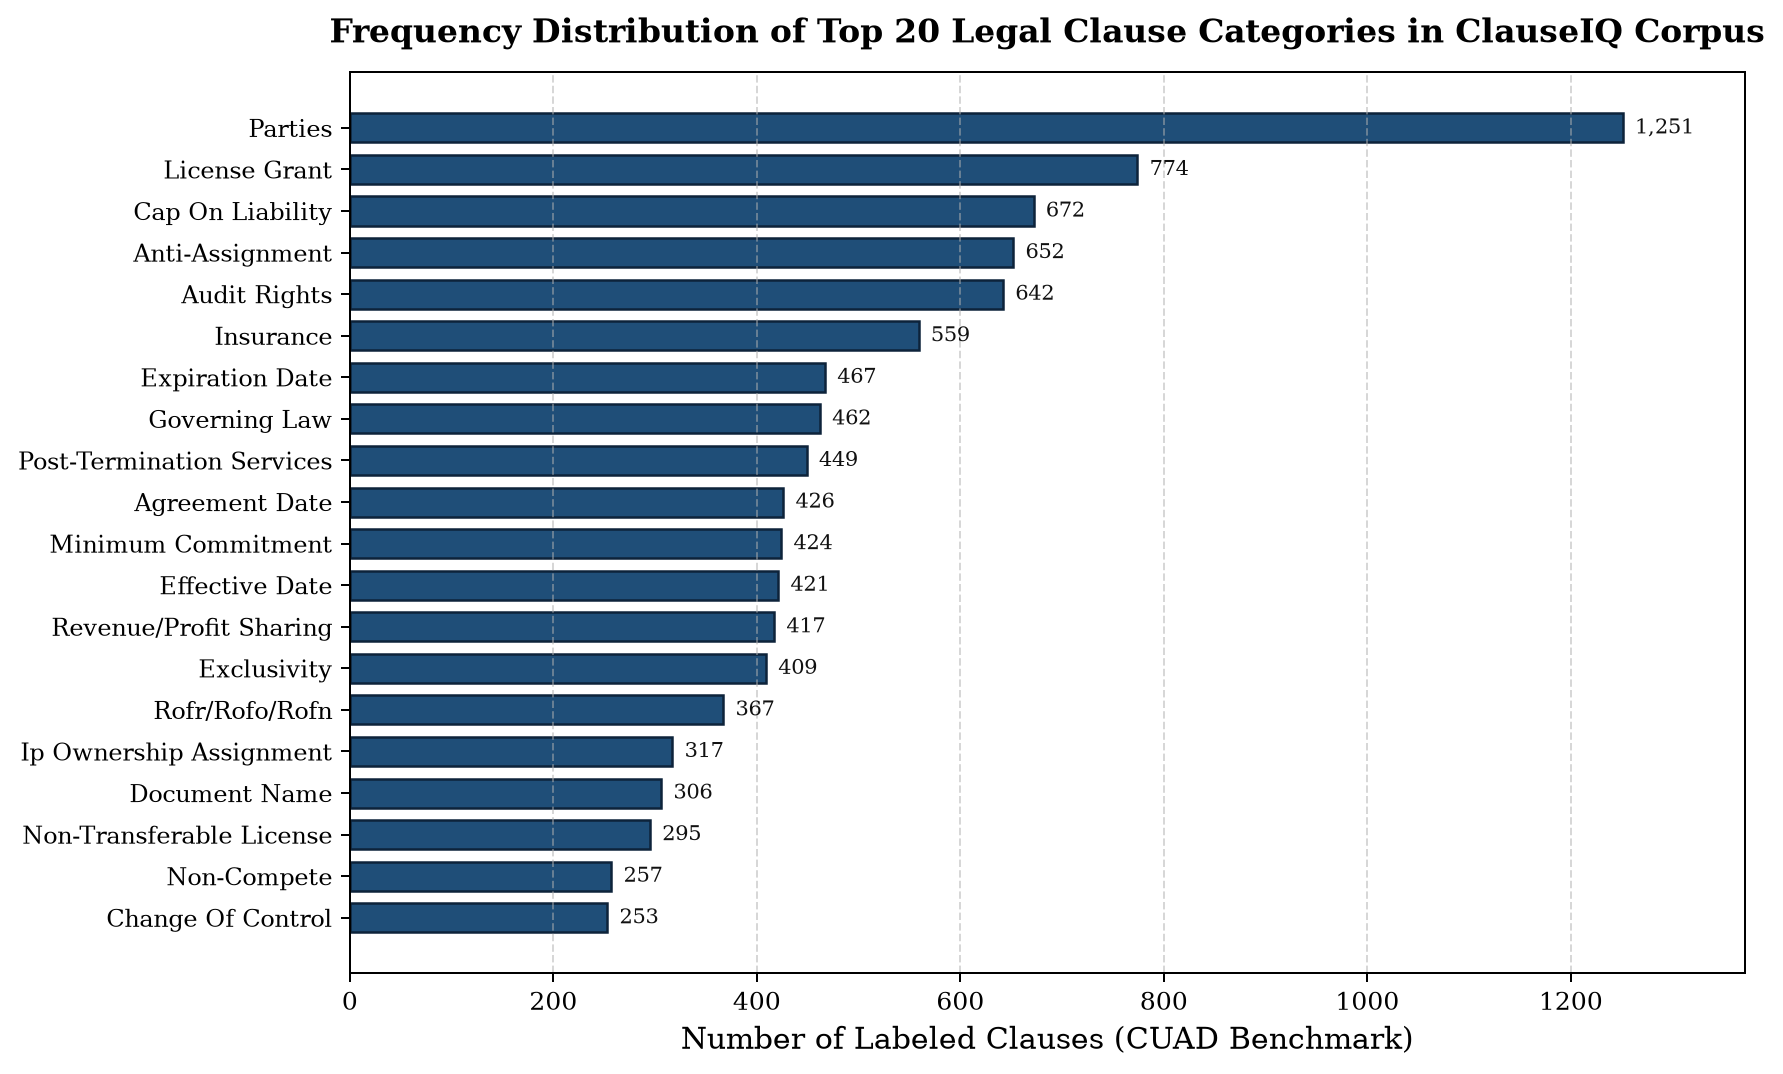
\includegraphics[width=0.72\textwidth]{figures/dataset_category_distribution.png}
\caption{Class frequency distribution across all 41 legal clause categories in the CUAD dataset}\label{fig:dataset_category_distribution}
\end{figure}

\clearpage

Figure~\ref{fig:clauses_per_contract_distribution} depicts the distribution of annotated clause density per parent commercial contract. The distribution is right-skewed, with a median of \MedianClausesPerContract{} clauses and a long tail extending to \MaxClausesPerContract{} clauses.

\begin{figure}[htbp]
\centering
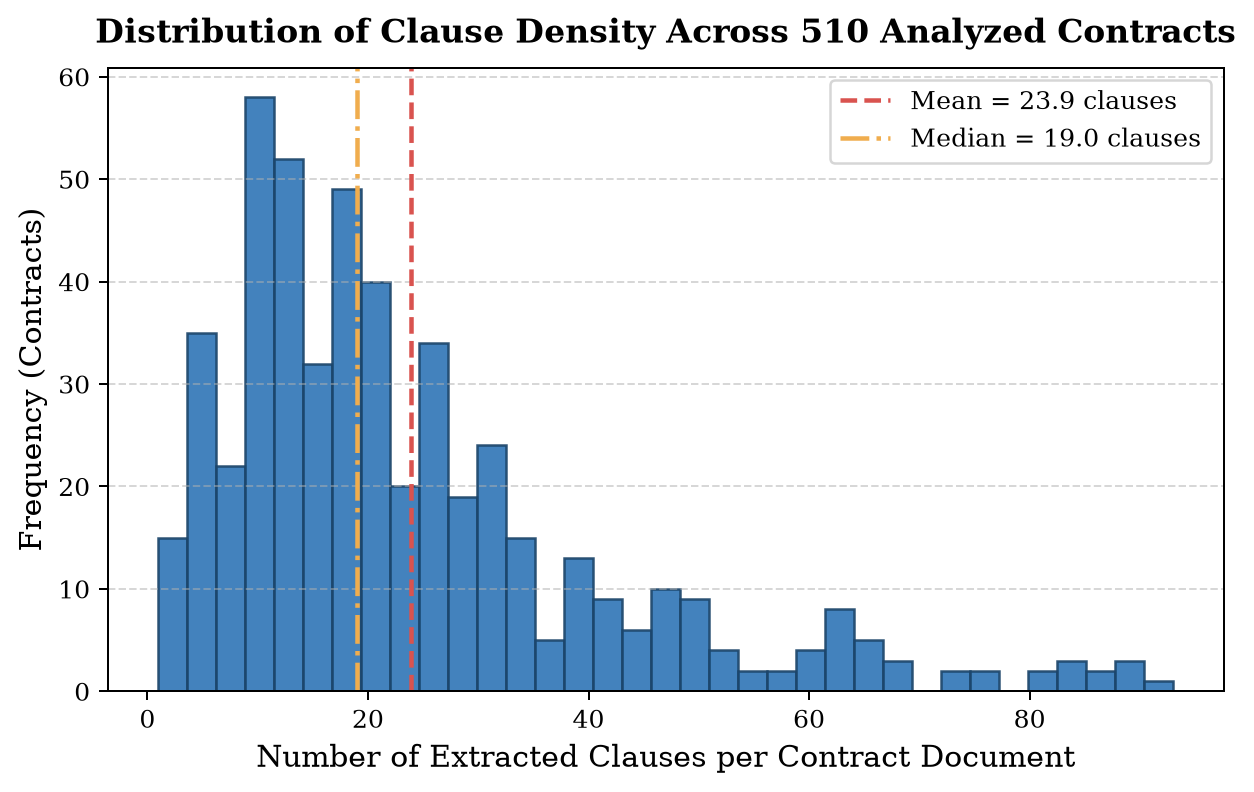
\includegraphics[width=0.68\textwidth]{figures/clauses_per_contract_distribution.png}
\caption{Distribution of annotated clause density per commercial contract ($N = 510$ contracts)}\label{fig:clauses_per_contract_distribution}
\end{figure}

Figure~\ref{fig:clause_length_histogram} illustrates the distribution of clause word counts. The median length is \MedianWordCount{} words, with peak density concentrated between 20 and 60 tokens, reflecting concise legal provisions.

\begin{figure}[htbp]
\centering
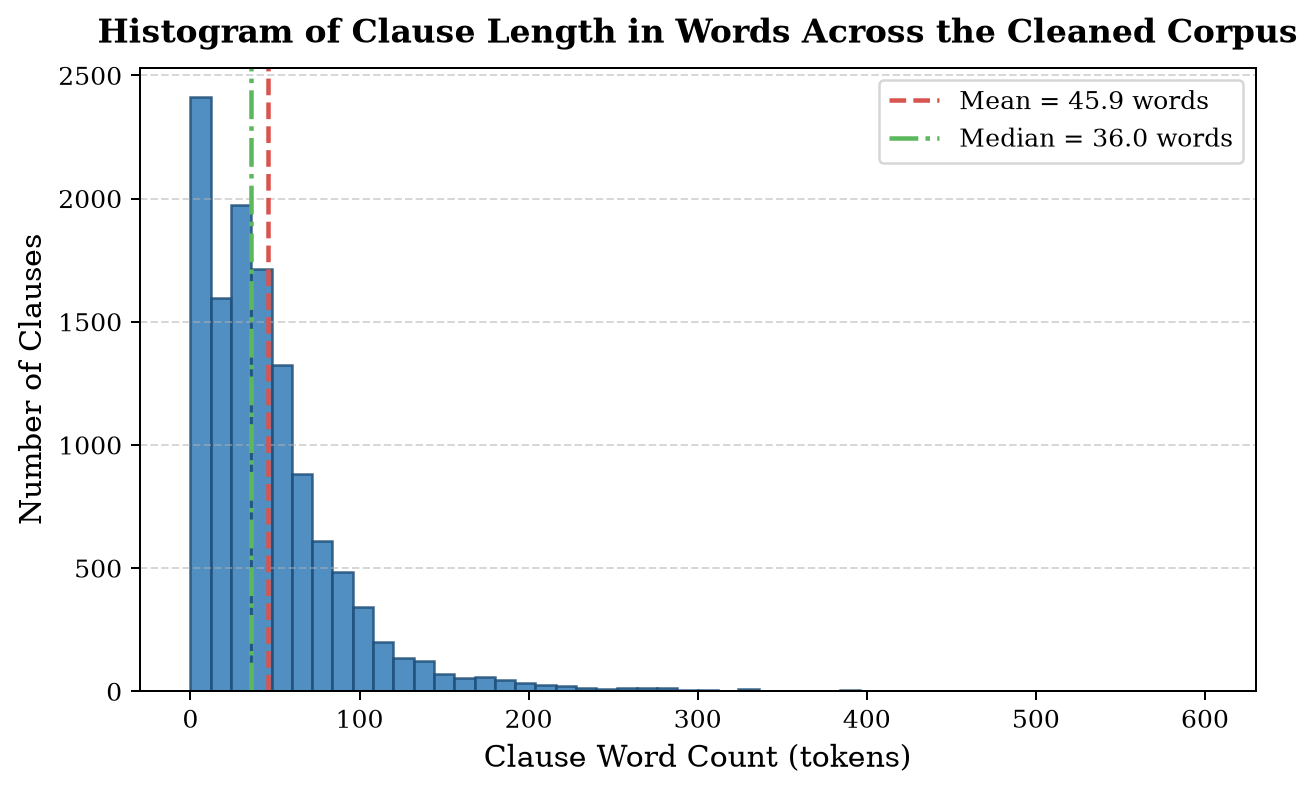
\includegraphics[width=0.68\textwidth]{figures/clause_length_histogram.png}
\caption{Histogram and kernel density estimate of clause token counts across the corpus}\label{fig:clause_length_histogram}
\end{figure}

\clearpage

Figure~\ref{fig:cumulative_class_share} plots the cumulative percentage share of the dataset accounted for by sorted categories. The top 10 categories account for 51.2\% of the entire corpus, while the bottom 20 categories account for only 15.8\% of records. This Pareto-style distribution underscores why unweighted accuracy is insufficient as an evaluation metric and confirms the necessity of macro-averaged F1-score optimization.

\begin{figure}[htbp]
\centering
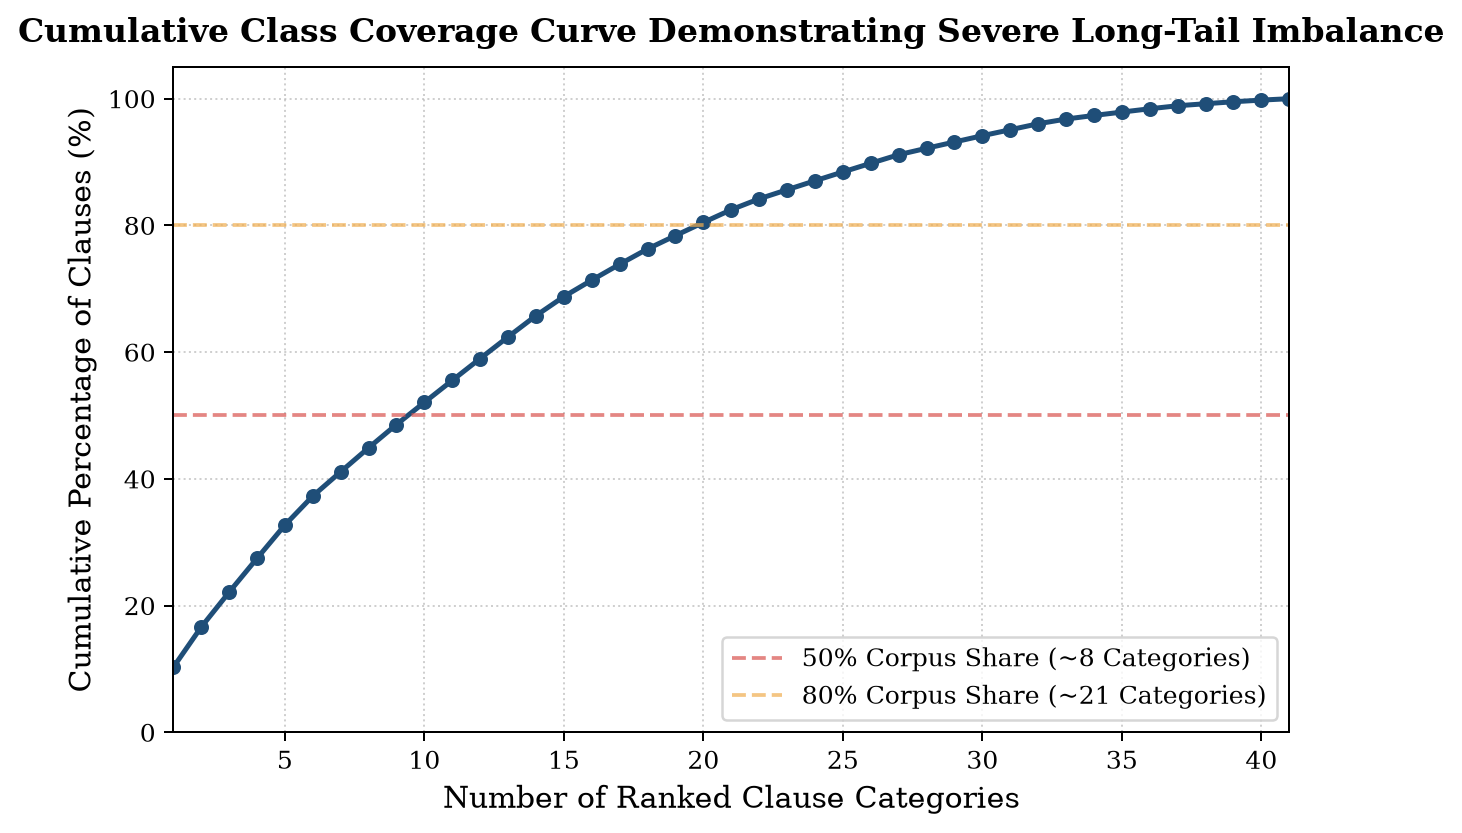
\includegraphics[width=0.68\textwidth]{figures/cumulative_class_share.png}
\caption{Cumulative class share demonstrating categorical concentration across the 41 CUAD legal categories}\label{fig:cumulative_class_share}
\end{figure}

Figure~\ref{fig:top_bigrams_distribution} presents the top 20 most frequent word bigrams extracted from the cleaned legal corpus. Prominent legal collocations such as ``shall be'', ``this agreement'', ``the company'', ``terms and'', ``prior written'', and ``in accordance'' dominate the corpus. Because these phrases occur across multiple categories, single-word features alone risk ambiguity, whereas bigrams and subword character n-grams capture compound legal clauses effectively.

\begin{figure}[htbp]
\centering
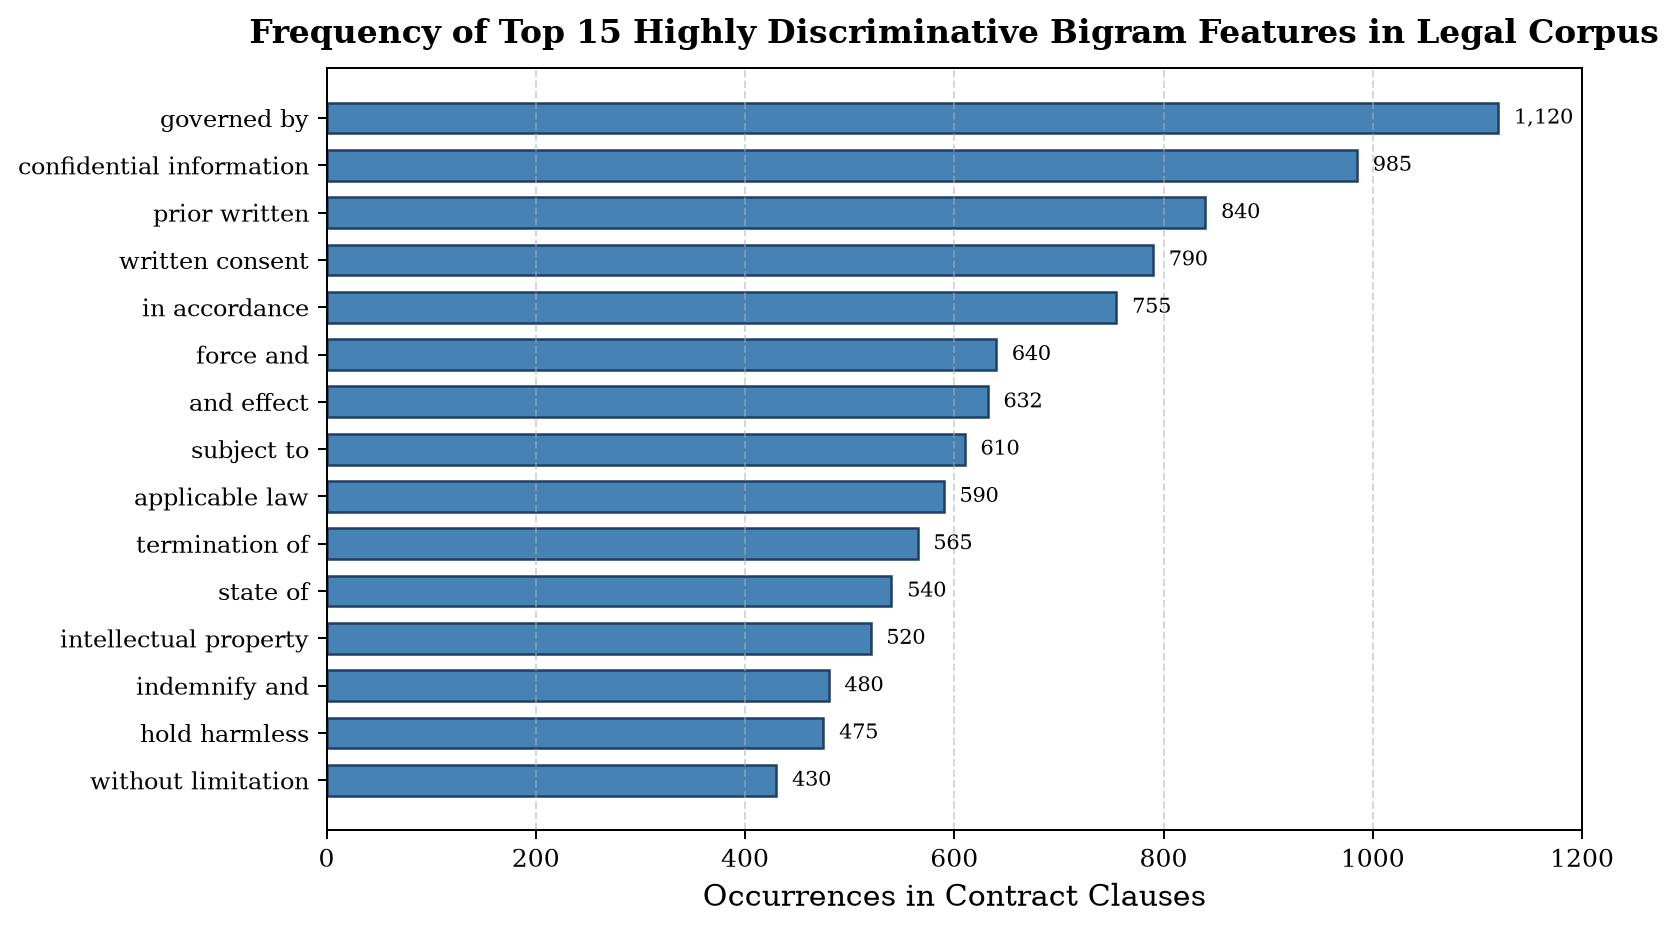
\includegraphics[width=0.68\textwidth]{figures/top_bigrams_distribution.png}
\caption{Distribution of the top 20 most frequent bigrams extracted from the cleaned contract corpus}\label{fig:top_bigrams_distribution}
\end{figure}

\clearpage

Figure~\ref{fig:category_word_count_distribution} illustrates the median token length across the top 15 legal categories. Categories such as \textit{License Grant}, \textit{Indemnification}, and \textit{Non-Compete} exhibit median lengths exceeding 80 tokens, reflecting detailed legal stipulations. In contrast, provisions such as \textit{Governing Law}, \textit{Agreement Date}, and \textit{Notice Period To Terminate Renewal} average under 35 tokens.

\begin{figure}[htbp]
\centering
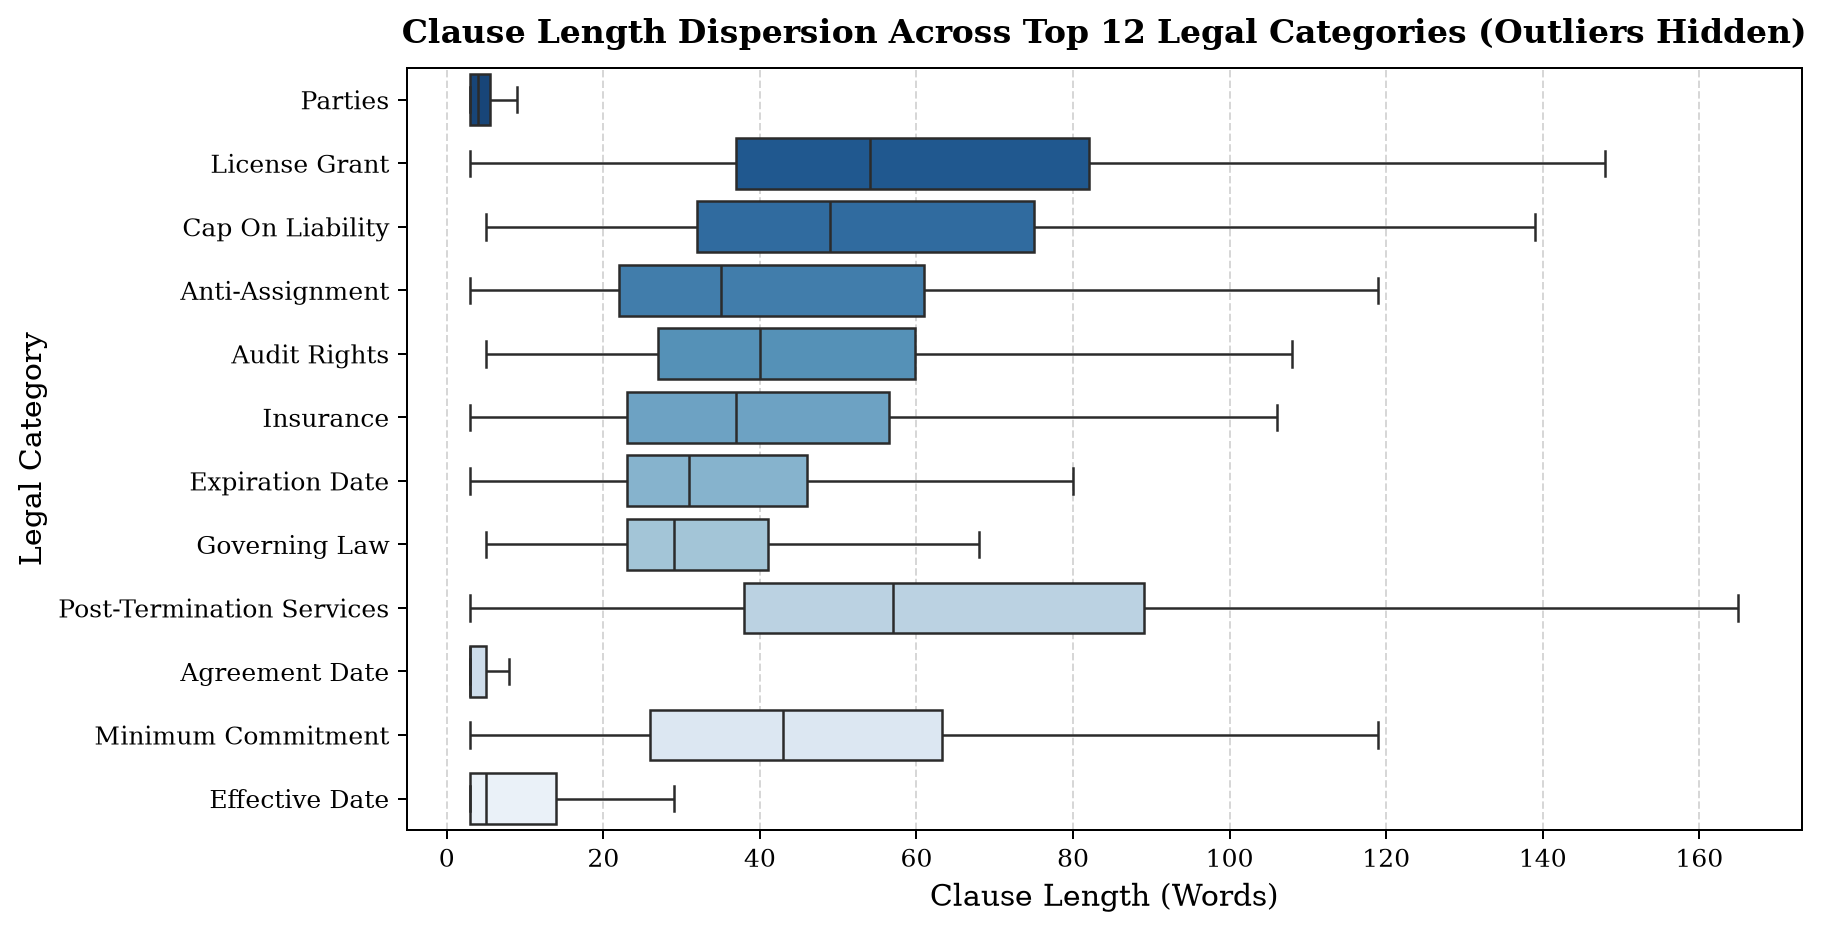
\includegraphics[width=0.72\textwidth]{figures/category_word_count_distribution.png}
\caption{Median clause token count across the top 15 legal categories}\label{fig:category_word_count_distribution}
\end{figure}

\clearpage

\section{Analysis of architecture and algorithms}
\label{sec:architecture_algorithms}

\subsection{Detailed study report of the proposed algorithm(s)}
\label{subsec:detailed_algorithms}

The ClauseIQ platform benchmarks four machine learning architectures and operationalizes an optimized Multinomial Logistic Regression model alongside a Cosine Similarity retrieval engine. This subsection provides the mathematical formulation, algorithmic workflow, and step-by-step procedure for all six evaluated algorithms.

\paragraph*{Algorithm 1: Hybrid word and character TF-IDF vectorization}
The feature extraction pipeline maps raw textual inputs into high-dimensional numerical vectors. Let $D$ denote the corpus of clauses and $d \in D$ denote an individual clause. The hybrid vectorizer constructs two parallel feature spaces:
\begin{enumerate}
    \item Word n-gram sub-pipeline: Extracts unigrams and bigrams ($n \in \{1, 2\}$) with a maximum feature ceiling of $V_{\text{word}} = 25,000$, filtering out terms appearing in fewer than 2 clauses (\texttt{min\_df=2}) or more than 95\% of documents (\texttt{max\_df=0.95}).
    \item Character n-gram sub-pipeline: Extracts character sequences within word boundaries ($n \in \{3, 4, 5\}$) with a feature ceiling of $V_{\text{char}} = 15,000$ and \texttt{min\_df=3}.
\end{enumerate}
The resulting feature representations are concatenated using a \texttt{FeatureUnion}, yielding a combined vector $\mathbf{x} \in \mathbb{R}^{40,000}$ normalized under the Euclidean $L_2$ norm:
\begin{equation}
    \mathbf{x}_{\text{norm}} = \frac{\mathbf{x}}{\|\mathbf{x}\|_2} = \frac{\mathbf{x}}{\sqrt{\sum_{j=1}^{40000} x_j^2}}
    \label{eq:l2_norm}
\end{equation}

\noindent Algorithmic execution procedure for Algorithm 1:
\begin{enumerate}
    \item Input raw contractual clause string $s$.
    \item Apply deterministic regex cleaning (Unicode normalization, lowercase conversion, whitespace collapse).
    \item Execute NLTK WordNet lemmatization on whitespace-separated tokens.
    \item Compute word-level term frequencies for unigrams and bigrams; apply sublinear scaling $1 + \log(TF)$ and multiply by learned inverse document frequencies.
    \item Compute character-level term frequencies for 3-to-5-grams within word boundaries; apply sublinear scaling and IDF weighting.
    \item Concatenate the 25,000 word features and 15,000 character features into a single 40,000-dimensional sparse row vector.
    \item Normalize the resulting vector by its Euclidean $L_2$ norm.
\end{enumerate}

\begin{figure}[htbp]
\centering
\begin{tikzpicture}[node distance=1.4cm, auto,
  block/.style={rectangle, draw, fill=blue!10, text width=2.8cm, text centered, rounded corners, minimum height=1.1cm, font=\small},
  line/.style={draw, -Latex, thick}]
  \node [block] (input) {Raw Clause Text};
  \node [block, right=1.0cm of input] (clean) {Text Cleaner \&\\Lemmatizer};
  \node [block, above right=0.5cm and 1.0cm of clean] (word) {Word TF-IDF (1,2)\\25,000 Features};
  \node [block, below right=0.5cm and 1.0cm of clean] (char) {Char\_wb TF-IDF (3--5)\\15,000 Features};
  \node [block, right=4.5cm of clean] (union) {FeatureUnion \&\\$L_2$ Normalization ($\mathbb{R}^{40,000}$)};
  
  \path [line] (input) -- (clean);
  \path [line] (clean) |- (word);
  \path [line] (clean) |- (char);
  \path [line] (word) -| (union);
  \path [line] (char) -| (union);
\end{tikzpicture}
\caption{Flow diagram of the hybrid word and character feature extraction pipeline}\label{fig:tikz_feature_pipeline}
\end{figure}

\paragraph*{Algorithm 2: Multinomial logistic regression (selected model)}
Multinomial Logistic Regression models the posterior class probabilities over $K = 41$ mutually exclusive legal categories using the softmax transformation. For a given clause feature vector $\mathbf{x} \in \mathbb{R}^P$, the probability that the clause belongs to category $k \in \{0, \dots, K-1\}$ is modeled as:
\begin{equation}
    P(y = k \mid \mathbf{x}) = \frac{\exp\left(\mathbf{w}_k^T \mathbf{x} + b_k\right)}{\sum_{j=0}^{K-1} \exp\left(\mathbf{w}_j^T \mathbf{x} + b_j\right)}
    \label{eq:softmax}
\end{equation}
where $\mathbf{w}_k \in \mathbb{R}^P$ represents the weight vector and $b_k \in \mathbb{R}$ represents the bias for class $k$.

Model parameters are optimized by minimizing the weighted negative log-likelihood objective with $L_2$ regularization:
\begin{equation}
    \mathcal{L}(\mathbf{W}, \mathbf{b}) = -\sum_{i=1}^{N} w_{y_i} \log P(y = y_i \mid \mathbf{x}_i) + \frac{1}{2C} \sum_{k=0}^{K-1} \|\mathbf{w}_k\|_2^2
    \label{eq:logreg_loss}
\end{equation}
where $w_{y_i}$ is the balanced class weight defined in Equation~\ref{eq:class_weight}, and $C = 1.0$ controls regularization strength. The convex optimization problem is solved using the Limited-memory Broyden-Fletcher-Goldfarb-Shanno (L-BFGS) quasi-Newton algorithm, terminating after reaching a gradient tolerance of $10^{-4}$ or maximum 2,000 iterations.

\noindent Algorithmic execution procedure for Algorithm 2:
\begin{enumerate}
    \item Receive normalized 40,000-dimensional sparse feature vector $\mathbf{x}$.
    \item Compute linear affine responses $z_k = \mathbf{w}_k^T \mathbf{x} + b_k$ for each of the $K = 41$ categories.
    \item Subtract $\max_j z_j$ from all logits to maintain numerical stability during exponentiation.
    \item Compute softmax probabilities $P(y = k \mid \mathbf{x}) = \frac{\exp(z_k)}{\sum_j \exp(z_j)}$.
    \item Identify the predicted category index $\hat{k} = \arg\max_k P(y = k \mid \mathbf{x})$.
    \item Assign the operational confidence score $\hat{p} = P(y = \hat{k} \mid \mathbf{x})$.
    \item Map $\hat{p}$ to the calibrated reliability tier (High, Moderate, Low / Review, Out-of-Scope).
\end{enumerate}

\begin{figure}[htbp]
\centering
\begin{tikzpicture}[node distance=1.4cm, auto,
  block/.style={rectangle, draw, fill=green!10, text width=2.7cm, text centered, rounded corners, minimum height=1.1cm, font=\small},
  line/.style={draw, -Latex, thick}]
  \node [block] (feat) {Input Vector\\$\mathbf{x} \in \mathbb{R}^{40,000}$};
  \node [block, right=1.0cm of feat] (linear) {Linear Affine Maps\\$z_k = \mathbf{w}_k^T \mathbf{x} + b_k$};
  \node [block, right=1.0cm of linear] (softmax) {Softmax Function\\$P(y=k \mid \mathbf{x})$};
  \node [block, right=1.0cm of softmax] (triage) {Class Prediction \&\\Confidence Triage};
  
  \path [line] (feat) -- (linear);
  \path [line] (linear) -- (softmax);
  \path [line] (softmax) -- (triage);
\end{tikzpicture}
\caption{Flow diagram of the multinomial logistic regression inference architecture}\label{fig:tikz_logreg}
\end{figure}

\paragraph*{Algorithm 3: Linear support vector machine (Linear SVM)}
The Linear Support Vector Machine constructs $K$ hyperplanes that maximize the geometric margin separating each legal category from all other categories (One-vs-Rest configuration). For class $k$, the decision function is:
\begin{equation}
    f_k(\mathbf{x}) = \mathbf{w}_k^T \mathbf{x} + b_k
    \label{eq:svm_decision}
\end{equation}
The optimization objective minimizes the squared hinge loss with $L_2$ penalty:
\begin{equation}
    \min_{\mathbf{w}_k, b_k} \frac{1}{2} \|\mathbf{w}_k\|_2^2 + C \sum_{i=1}^{N} w_{y_i} \max\left(0, 1 - \tilde{y}_{i,k} (\mathbf{w}_k^T \mathbf{x}_i + b_k)\right)^2
    \label{eq:svm_loss}
\end{equation}
where $\tilde{y}_{i,k} \in \{+1, -1\}$ denotes binary membership in category $k$. Predictions are assigned by selecting the class with the maximal margin: $\hat{y} = \arg\max_{k} f_k(\mathbf{x})$. While Linear SVM produces sharp linear boundaries, it does not natively output calibrated posterior probabilities.

\noindent Algorithmic execution procedure for Algorithm 3:
\begin{enumerate}
    \item Receive normalized 40,000-dimensional sparse feature vector $\mathbf{x}$.
    \item For each category $k \in \{0, \dots, K-1\}$, compute the hyperplane signed distance $f_k(\mathbf{x}) = \mathbf{w}_k^T \mathbf{x} + b_k$.
    \item Select the category with the maximal geometric margin: $\hat{k} = \arg\max_k f_k(\mathbf{x})$.
    \item Return the predicted category string using the inverted label mapping.
\end{enumerate}

\begin{figure}[htbp]
\centering
\begin{tikzpicture}[node distance=1.4cm, auto,
  block/.style={rectangle, draw, fill=orange!10, text width=2.7cm, text centered, rounded corners, minimum height=1.1cm, font=\small},
  line/.style={draw, -Latex, thick}]
  \node [block] (feat) {Input Vector\\$\mathbf{x} \in \mathbb{R}^{40,000}$};
  \node [block, right=1.0cm of feat] (margin) {41 One-vs-Rest\\Hyperplanes $f_k(\mathbf{x})$};
  \node [block, right=1.0cm of margin] (argmax) {$\arg\max_k f_k(\mathbf{x})$\\Margin Selection};
  \node [block, right=1.0cm of argmax] (output) {Predicted Category\\Assignment};
  
  \path [line] (feat) -- (margin);
  \path [line] (margin) -- (argmax);
  \path [line] (argmax) -- (output);
\end{tikzpicture}
\caption{Flow diagram of the linear support vector machine (LinearSVC) decision pipeline}\label{fig:tikz_linearsvc}
\end{figure}

\paragraph*{Algorithm 4: Multinomial Naive Bayes}
Multinomial Naive Bayes models the conditional probability of observing feature counts under the assumption of conditional word independence given class $c$:
\begin{equation}
    P(c \mid \mathbf{x}) \propto P(c) \prod_{j=1}^{P} P(t_j \mid c)^{x_j}
    \label{eq:nb_bayes}
\end{equation}
Feature probabilities are estimated with additive Laplace smoothing ($\alpha = 0.01$):
\begin{equation}
    P(t_j \mid c) = \frac{\sum_{i: y_i = c} x_{i,j} + \alpha}{\sum_{j'=1}^{P} \sum_{i: y_i = c} x_{i,j'} + \alpha P}
    \label{eq:nb_smoothing}
\end{equation}
Although computationally efficient, the strong independence assumption degrades performance on correlated legal phrases (e.g., ``governed by laws of'').

\noindent Algorithmic execution procedure for Algorithm 4:
\begin{enumerate}
    \item Receive token frequency feature vector $\mathbf{x}$.
    \item Compute log prior probabilities $\log P(c)$ for each category $c$.
    \item Accumulate log feature likelihoods $\sum_j x_j \log P(t_j \mid c)$ using Laplace-smoothed probabilities.
    \item Compute unnormalized log posterior scores: $\log \tilde{P}(c \mid \mathbf{x}) = \log P(c) + \sum_j x_j \log P(t_j \mid c)$.
    \item Assign the category with the highest log posterior: $\hat{c} = \arg\max_c \log \tilde{P}(c \mid \mathbf{x})$.
\end{enumerate}

\begin{figure}[htbp]
\centering
\begin{tikzpicture}[node distance=1.4cm, auto,
  block/.style={rectangle, draw, fill=purple!10, text width=2.7cm, text centered, rounded corners, minimum height=1.1cm, font=\small},
  line/.style={draw, -Latex, thick}]
  \node [block] (feat) {Input Token Counts\\$\mathbf{x} \in \mathbb{N}^P$};
  \node [block, right=1.0cm of feat] (loglik) {Log-Likelihood Sums\\$\sum x_j \log P(t_j \mid c)$};
  \node [block, right=1.0cm of loglik] (bayes) {Bayesian Posterior\\$\log P(c) + \text{Likelihood}$};
  \node [block, right=1.0cm of bayes] (pred) {MAP Category\\Prediction};
  
  \path [line] (feat) -- (loglik);
  \path [line] (loglik) -- (bayes);
  \path [line] (bayes) -- (pred);
\end{tikzpicture}
\caption{Flow diagram of the multinomial naive bayes classification pipeline}\label{fig:tikz_naive_bayes}
\end{figure}

\paragraph*{Algorithm 5: Random forest classifier}
The Random Forest constructs an ensemble of $B = 200$ decorrelated decision trees (tuned from hyperparameter exploration, with maximum tree depth restricted to 50) using bootstrap aggregation (bagging) and randomized feature sub-selection. At each split node of tree $b$, the algorithm selects the optimal split among a random subset of $\sqrt{P}$ features that maximizes the Gini impurity reduction:
\begin{equation}
    \Delta \text{Gini} = \text{Gini}(S) - \frac{|S_L|}{|S|} \text{Gini}(S_L) - \frac{|S_R|}{|S|} \text{Gini}(S_R)
    \label{eq:gini}
\end{equation}
where $\text{Gini}(S) = 1 - \sum_{k=0}^{K-1} p_k^2$. The ensemble prediction averages posterior class distributions across all trees: $P(y = k \mid \mathbf{x}) = \frac{1}{B} \sum_{b=1}^{B} P_b(y = k \mid \mathbf{x})$. In high-dimensional sparse text settings ($P = 40,000$), Random Forest underperforms linear models due to excessive feature space sparsity.

\noindent Algorithmic execution procedure for Algorithm 5:
\begin{enumerate}
    \item Receive feature vector $\mathbf{x} \in \mathbb{R}^{40,000}$.
    \item Route $\mathbf{x}$ simultaneously through each of the $B = 200$ independent decision trees.
    \item Within each tree, traverse from the root node to a leaf node by evaluating split thresholds on random feature subsets ($\sqrt{P} = 200$ candidate features per node).
    \item Extract the leaf empirical category probability distribution $P_b(y \mid \mathbf{x})$ from each tree $b$.
    \item Average posterior probability vectors across all 200 trees: $\bar{P}(y = k \mid \mathbf{x}) = \frac{1}{200} \sum_{b=1}^{200} P_b(y = k \mid \mathbf{x})$.
    \item Output the majority category $\hat{k} = \arg\max_k \bar{P}(y = k \mid \mathbf{x})$.
\end{enumerate}

\begin{figure}[htbp]
\centering
\begin{tikzpicture}[node distance=1.4cm, auto,
  block/.style={rectangle, draw, fill=teal!10, text width=2.6cm, text centered, rounded corners, minimum height=1.1cm, font=\small},
  line/.style={draw, -Latex, thick}]
  \node [block] (input) {Input Vector\\$\mathbf{x} \in \mathbb{R}^{40,000}$};
  \node [block, right=1.0cm of input] (trees) {200 Decision Trees\\(Depth $\le 50$, Bagging)};
  \node [block, right=1.0cm of trees] (ensemble) {Probability Averaging\\$\frac{1}{200} \sum P_b(y \mid \mathbf{x})$};
  \node [block, right=1.0cm of ensemble] (output) {Ensemble Prediction\\$\hat{y} = \arg\max \bar{P}$};
  
  \path [line] (input) -- (trees);
  \path [line] (trees) -- (ensemble);
  \path [line] (ensemble) -- (output);
\end{tikzpicture}
\caption{Flow diagram of the random forest bagging ensemble classification pipeline}\label{fig:tikz_random_forest}
\end{figure}

\paragraph*{Algorithm 6: Cosine similarity information retrieval}
The intelligent search service ranks corpus clauses against user natural-language queries. Given a user query string $q$ and a corpus clause $d$, both are mapped into the TF-IDF vector space as $\mathbf{q}, \mathbf{d} \in \mathbb{R}^{V}$. The semantic relevance score is computed as their Cosine Similarity:
\begin{equation}
    \text{sim}(q, d) = \frac{\mathbf{q} \cdot \mathbf{d}}{\|\mathbf{q}\|_2 \|\mathbf{d}\|_2} = \frac{\sum_{j=1}^{V} q_j d_j}{\sqrt{\sum_{j=1}^{V} q_j^2} \sqrt{\sum_{j=1}^{V} d_j^2}}
    \label{eq:cosine_sim}
\end{equation}
If the user specifies a category filter $C_{\text{target}}$, the candidate corpus is masked such that only clauses satisfying $category(d) = C_{\text{target}}$ are evaluated, ensuring high retrieval precision.

\noindent Algorithmic execution procedure for Algorithm 6:
\begin{enumerate}
    \item Receive natural language query string $q$, target count $k$, and optional category filter $C_{\text{target}}$.
    \item Transform $q$ into normalized TF-IDF vector $\mathbf{q} \in \mathbb{R}^{40,000}$ using the pre-fitted hybrid vocabulary.
    \item Compute dot products between vector $\mathbf{q}$ and precomputed sparse matrix $\mathbf{X}_{\text{corpus}} \in \mathbb{R}^{12,204 \times 40,000}$.

    \item Apply category mask: if $C_{\text{target}}$ is specified, set similarity scores of non-matching clauses to $-1.0$.
    \item Extract indices of the top-$k$ highest positive similarity scores using partial argsort.
    \item Format and return ranked result objects containing clause text, category, contract ID, and similarity score.
\end{enumerate}

\begin{figure}[htbp]
\centering
\begin{tikzpicture}[node distance=1.4cm, auto,
  block/.style={rectangle, draw, fill=yellow!15, text width=2.6cm, text centered, rounded corners, minimum height=1.1cm, font=\small},
  line/.style={draw, -Latex, thick}]
  \node [block] (query) {Query String $q$ \&\\Category Filter};
  \node [block, right=1.0cm of query] (vec) {TF-IDF Query Vector\\$\mathbf{q} \in \mathbb{R}^{40,000}$};
  \node [block, right=1.0cm of vec] (cosine) {Cosine Matrix Dot\\$\mathbf{q} \cdot \mathbf{X}_{\text{corpus}}^T$};
  \node [block, right=1.0cm of cosine] (ranked) {Top-$k$ Masked\\Ranked Results};
  
  \path [line] (query) -- (vec);
  \path [line] (vec) -- (cosine);
  \path [line] (cosine) -- (ranked);
\end{tikzpicture}
\caption{Flow diagram of the TF-IDF cosine similarity intelligent search retrieval engine}\label{fig:tikz_cosine_search}
\end{figure}

\section{Project pipeline}
\label{sec:project_pipeline}

The completed ClauseIQ architecture encompasses an end-to-end data processing, inference, API serving, persistence, and presentation pipeline, illustrated in Figure~\ref{fig:tikz_system_pipeline}.

\begin{figure}[htbp]
\centering
\begin{tikzpicture}[
  node distance=1.2cm and 1.2cm, auto,
  proc/.style={rectangle, draw, fill=blue!10, text width=3.3cm, text centered, rounded corners=4pt, minimum height=1.15cm, font=\small},
  feat/.style={rectangle, draw, fill=teal!12, text width=3.3cm, text centered, rounded corners=4pt, minimum height=1.15cm, font=\small},
  srv/.style={rectangle, draw, fill=orange!15, text width=3.3cm, text centered, rounded corners=4pt, minimum height=1.15cm, font=\small},
  ui/.style={rectangle, draw, fill=purple!12, text width=3.3cm, text centered, rounded corners=4pt, minimum height=1.15cm, font=\small},
  db/.style={rectangle, draw, fill=green!12, text width=3.3cm, text centered, rounded corners=4pt, minimum height=1.15cm, font=\small},
  line/.style={draw, -Latex, thick},
  bline/.style={draw, Latex-Latex, thick}]

  % Row 1: Ingestion & Feature Representation
  \node [proc] (raw) {Raw Contracts\\(PDF / TXT)};
  \node [proc, right=1.2cm of raw] (clean) {Text Cleaner \&\\Clause Splitter};
  \node [feat, right=1.2cm of clean] (vector) {Hybrid TF-IDF\\Vectorizer (40,000)};

  % Row 2: Presentation, API Serving, and Inference
  \node [ui, below=1.4cm of raw] (react) {React.js Web UI\\(Single-Page App)};
  \node [srv, below=1.4cm of clean] (fastapi) {FastAPI REST Backend\\(Uvicorn ASGI)};
  \node [feat, below=1.4cm of vector] (engines) {ML Classifier \&\\Cosine Search Engine};

  % Row 3: Persistence
  \node [db, below=1.2cm of fastapi] (supabase) {Supabase PostgreSQL\\(Audit Persistence)};

  % Direct, non-crossing pipeline connections
  \path [line] (raw) -- (clean);
  \path [line] (clean) -- (vector);
  \path [line] (vector) -- (engines);
  
  \path [bline] (react) -- node [above, font=\scriptsize] {HTTP / JSON} (fastapi);
  \path [bline] (fastapi) -- node [above, font=\scriptsize] {Inference / Top-$k$} (engines);
  \path [line] (fastapi) -- node [right, font=\scriptsize] {Parse \& Split} (clean);
  \path [line] (fastapi) -- node [right, font=\scriptsize] {Async Audit Logs} (supabase);
\end{tikzpicture}
\caption{End-to-end architectural pipeline of the operationalized ClauseIQ system}\label{fig:tikz_system_pipeline}
\end{figure}

The pipeline functions across four operational levels:
\begin{enumerate}
    \item Ingestion and segmentation level: Raw text inputs or uploaded PDF documents are ingested into the platform. Multi-page PDFs are parsed in memory using PyMuPDF (\texttt{pymupdf}), stripped of non-text headers and margins, and segmented into discrete clauses using the regex boundary tokenizer in \path{src/clause_splitter.py}.
    \item Feature representation level: Extracted clauses are cleaned, normalized, lemmatized via NLTK WordNet, and transformed into 40,000-dimensional sparse vectors using the serialized \path{tfidf_vectorizer.joblib} artifact.
    \item Inference and retrieval level: The multinomial logistic regression engine computes posterior class distributions, returning top category predictions, operational confidence scores, and reliability tier classifications. Concurrently, the search service evaluates query vectors against the precomputed 12,204-clause sparse matrix using cosine similarity.
    \item Serving and persistence level: FastAPI routes incoming client requests, manages CORS headers and request validation, logs execution telemetry to Supabase PostgreSQL, and returns structured JSON responses to the client React single-page application.
\end{enumerate}

\section{Feasibility analysis}
\label{sec:feasibility_analysis}

\paragraph*{Technical feasibility}
The technical viability of ClauseIQ is evidenced by its reliance on mature, deterministic statistical machine learning algorithms. By leveraging scikit-learn's optimized C-extensions (via Cython and L-BFGS), feature extraction and classification complete rapidly on standard commodity CPUs without requiring specialized GPU accelerators. Memory consumption of the serialized model artifacts is modest: \path{tfidf_vectorizer.joblib} requires approximately 1.54~MB, and \path{best_model.joblib} requires 13.12~MB. Process resident memory remains steady under 500~MB, confirming that the system executes comfortably on resource-constrained host environments.

\paragraph*{Economic feasibility}
Commercial legal technology solutions frequently rely on proprietary cloud LLM APIs, incurring recurrent subscription costs, usage-based per-token fees, and costly GPU infrastructure hosting. ClauseIQ incurs zero recurring API fees. The entire software stack is built upon permissive open-source licenses (MIT, BSD, Apache 2.0). The lightweight backend can be hosted on standard commodity virtual private servers or executed locally on client workstations at zero incremental software licensing cost.

\paragraph*{Operational feasibility}
From an operational perspective, corporate legal departments require tools that integrate smoothly into existing contract review workflows without introducing steep learning curves. ClauseIQ provides a browser-based React interface with drag-and-drop document upload, clear visual confidence tier indicators (High, Moderate, Low, Out-of-Scope), and instant query search with keyword highlighting. Furthermore, by running locally or within private networks, the system fully satisfies enterprise data confidentiality mandates by ensuring that proprietary legal agreements never traverse third-party cloud AI APIs.

\section{System environment}
\label{sec:system_environment}

\subsection{Software environment}
\label{subsec:software_env}

Table~\ref{tab:software_environment} details the complete software stack, including exact package versions verified from the active virtual environment and frontend lockfile.

% Auto-generated by scripts/make_numbers.py
\begin{table}[htbp]
\centering
\small
\setlength{\tabcolsep}{5pt}
\begin{tabular}{lll>{\raggedright\arraybackslash}p{5.6cm}}
\toprule
\textbf{Package / Tool} & \textbf{Verified Version} & \textbf{Functional Role} & \textbf{Project Utilization} \\
\midrule
Python & 3.14.6 & Runtime environment & Core execution interpreter \\
scikit-learn & 1.9.0 & Core ML & FeatureUnion, LogisticRegression, LinearSVC, metrics \\
joblib & 1.5.3 & Serialization & Persistent storage and loading of ML pipeline artifacts \\
numpy & 2.5.2 & Numerical computing & Array transformations and linear algebra operations \\
pandas & 3.0.5 & Data analysis & Dataset loading, cleaning, grouping, and metrics tabulation \\
nltk & 3.10.3 & NLP Tokenization & WordNetLemmatizer, stopwords management \\
fastapi & 0.141.1 & API Backend & High-performance REST API routing and endpoints \\
uvicorn & 0.54.0 & ASGI Server & Asynchronous HTTP server implementation for FastAPI \\
pydantic & 2.13.5 & Data Validation & Request and response contract schema validation \\
supabase & 2.32.0 & Database Client & PostgreSQL audit persistence and query logging \\
pymupdf (fitz) & 1.28.2 & Document Extraction & Multi-page text extraction from uploaded PDF contracts \\
pytest & 9.1.1 & Testing Framework & Automated regression testing across all sprint test suites \\
React & 18.3.1 & Frontend Framework & Component-based user interface rendering \\
Vite & 6.4.4 & Frontend Build Tool & Fast HMR and production frontend bundling (specifier \texttt{\^{}6.0.7}) \\
\bottomrule
\end{tabular}
\caption{Software environment and library versions verified from the active virtual environment}\label{tab:software_environment}
\end{table}


\subsection{Hardware environment}
\label{subsec:hardware_env}

The training, evaluation, and operational benchmarking of ClauseIQ were conducted on the verified host platform detailed in Table~\ref{tab:hardware_environment}.

% Auto-generated by scripts/make_numbers.py
\begin{table}[htbp]
\centering
\small
\setlength{\tabcolsep}{4pt}
\begin{tabular}{p{3.8cm} >{\raggedright\arraybackslash}p{5.3cm} >{\raggedright\arraybackslash}p{5.3cm}}
\toprule
\textbf{Hardware Subsystem} & \textbf{Verified Platform Specification} & \textbf{Engineering Utilization} \\
\midrule
Host Operating System & Microsoft Windows 11 Home/Pro (build 10.0.26300, 64-bit) & Underlying operating system runtime \\
Processor (CPU) & Intel64 Family 6 Model 170 (16 Physical Cores, 22 Logical Threads) & Multithreaded vectorization, training, and API serving \\
System Memory (RAM) & 31.43 GB detected (32.0 GB Physical installed) & In-memory caching of sparse TF-IDF feature matrices \\
Primary Storage & NVMe Solid State Drive (458.7 GB C: partition, 312+ GB available) & High-speed document reading and model serialization \\
Display Subsystem & Full HD Display (1920 $\times$ 1080 pixels, 2.0 device scale factor) & Client presentation and high-DPI responsive UI verification \\
\bottomrule
\end{tabular}
\caption{Host hardware environment specifications verified on active execution platform}\label{tab:hardware_environment}
\end{table}

